\begin{frame}[t]
\frametitle{The Execution Model}
  \begin{itemize}
    \item Several objects live on a single ``processor''
    \begin{itemize}
      \item We will come back to what we mean by a processor.
      \begin{itemize}
        \item For now, think of it as a core
      \end{itemize}
    \end{itemize}
  \pause
  \item As a result, 
    \begin{itemize}
      \item Method invocations directed at objects on that processor will have to be stored in a pool
      \pause
      \item And a user-level scheduler will select one invocation from the queue and runs it to completion
    \end{itemize}
  \end{itemize}
  \begin{center} 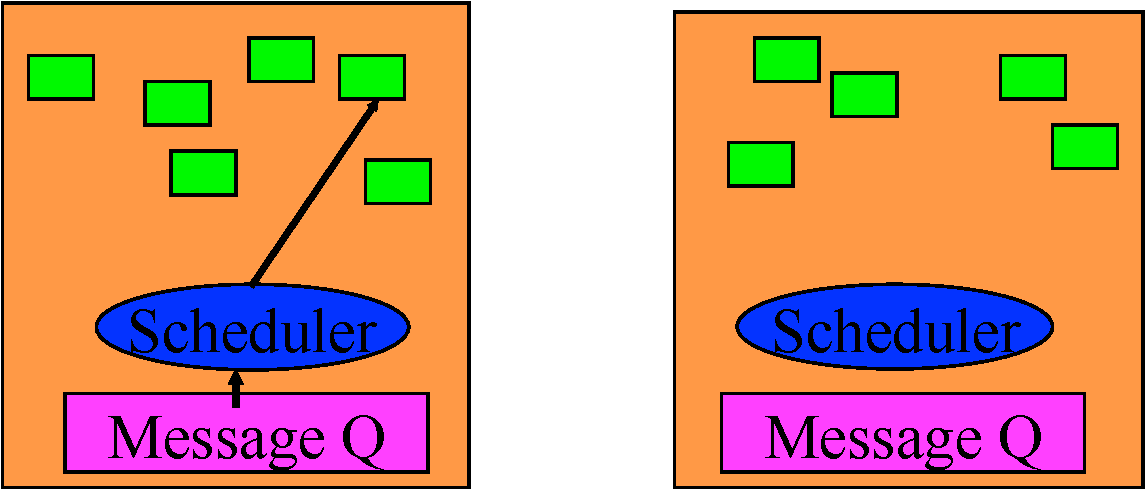
\includegraphics[width=0.7\textwidth]{figures/scheduler} \end{center}
\end{frame}

\begin{frame}[t]
\frametitle{Message-driven Execution}
  \begin{itemize}
    \item Execution is triggered by availability of a ``message'' (a method invocation)
    \pause
    \item When an entry method executes, 
    \begin{itemize}
      \item it may generate messages for other objects
      \item the RTS deposits them in the message Q on the target processor
    \end{itemize}
  \end{itemize}
  \begin{center} 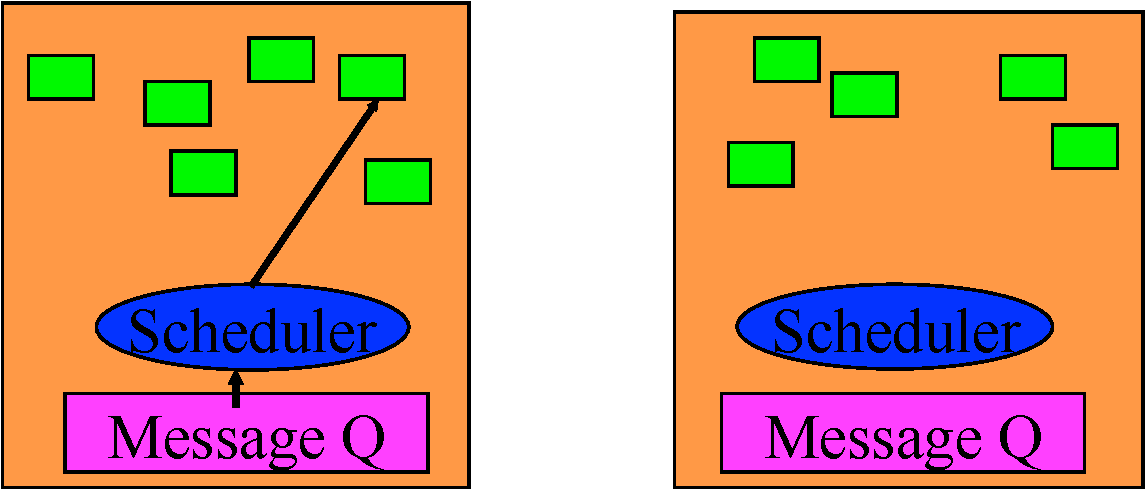
\includegraphics[width=0.7\textwidth]{figures/scheduler} \end{center}
\end{frame}

\begin{frame}[t]
\frametitle{Utility for Multi-cores, Many-cores, Accelerators}
  \begin{itemize}
    \item Objects connote and promote locality
    \item Message-driven execution is
    \begin{itemize}
      \item A strong principle of prediction for data and code use
      \item Much stronger than principle of locality
      \begin{itemize}
        \item Can be used to scale memory wall
        \item Prefetching of needed data, e.g, into scratch pad memories
      \end{itemize}
    \end{itemize}
  \end{itemize}
  \begin{center} 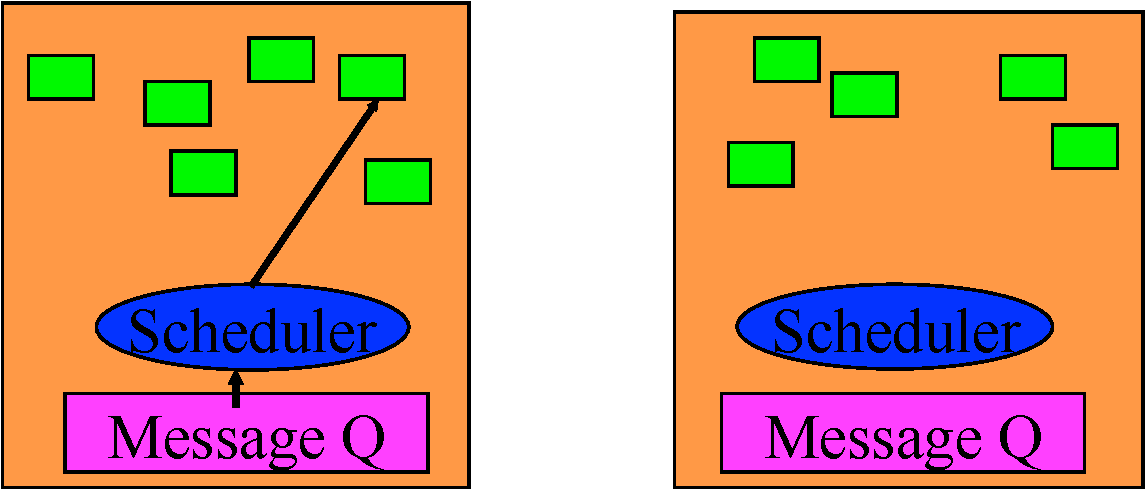
\includegraphics[width=0.7\textwidth]{figures/scheduler} \end{center}
\end{frame}

\begin{frame}[t]
\frametitle{Impact on communication}
  \begin{itemize}
    \item Current use of communication network
    \begin{itemize}
      \item Compute-communicate cycles in typical MPI apps
      \item Network is used for a fraction of time
      \item And is on the critical path
    \end{itemize}
    \pause
    \item Hence, current communication networks are over-engineered by necessity
    \pause
    \item With overdecomposition
    \begin{itemize}
      \item Communication is spread over an iteration
      \item Adaptive overlap of communication and computation
    \end{itemize}
  \end{itemize}
\end{frame}

\begin{frame}[t]
\frametitle{Example: Stencil Computation}
  \begin{itemize}
    \item Consider a simple stencil computation
    \begin{itemize}
      \item With traditional design based on traditional methods (e.g.  MPI-based)
      \begin{itemize}
        \item Each processor has a chunk, which alternates between computing and communicating
      \end{itemize}
      \pause
      \item With Charm++
      \begin{itemize}
        \item Multiple chunks on each processor
        \item Wait time for each chunk overlapped with useful computation for others
        \item Communication spread over time
      \end{itemize}
    \end{itemize}
  \end{itemize}
\end{frame}

\begin{frame}[t]
\frametitle{Example: Stencil Computation}
  \begin{center} 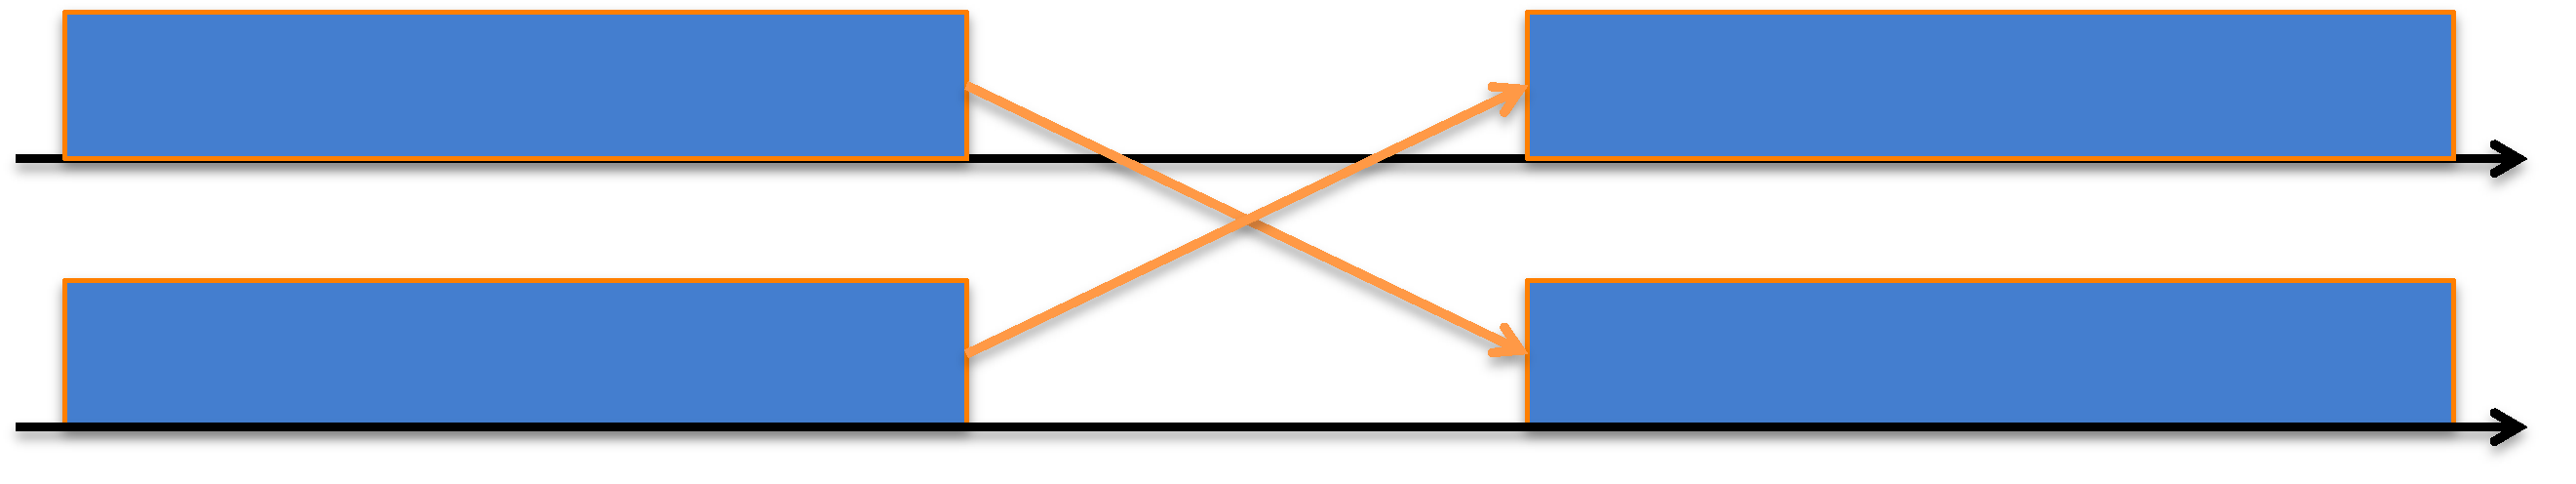
\includegraphics[width=\textwidth]{figures/stencil_timeline} \end{center}
  \begin{center} Stencil in MPI: No overlap among computation and
  communication\end{center}
  \pause
  \begin{center} 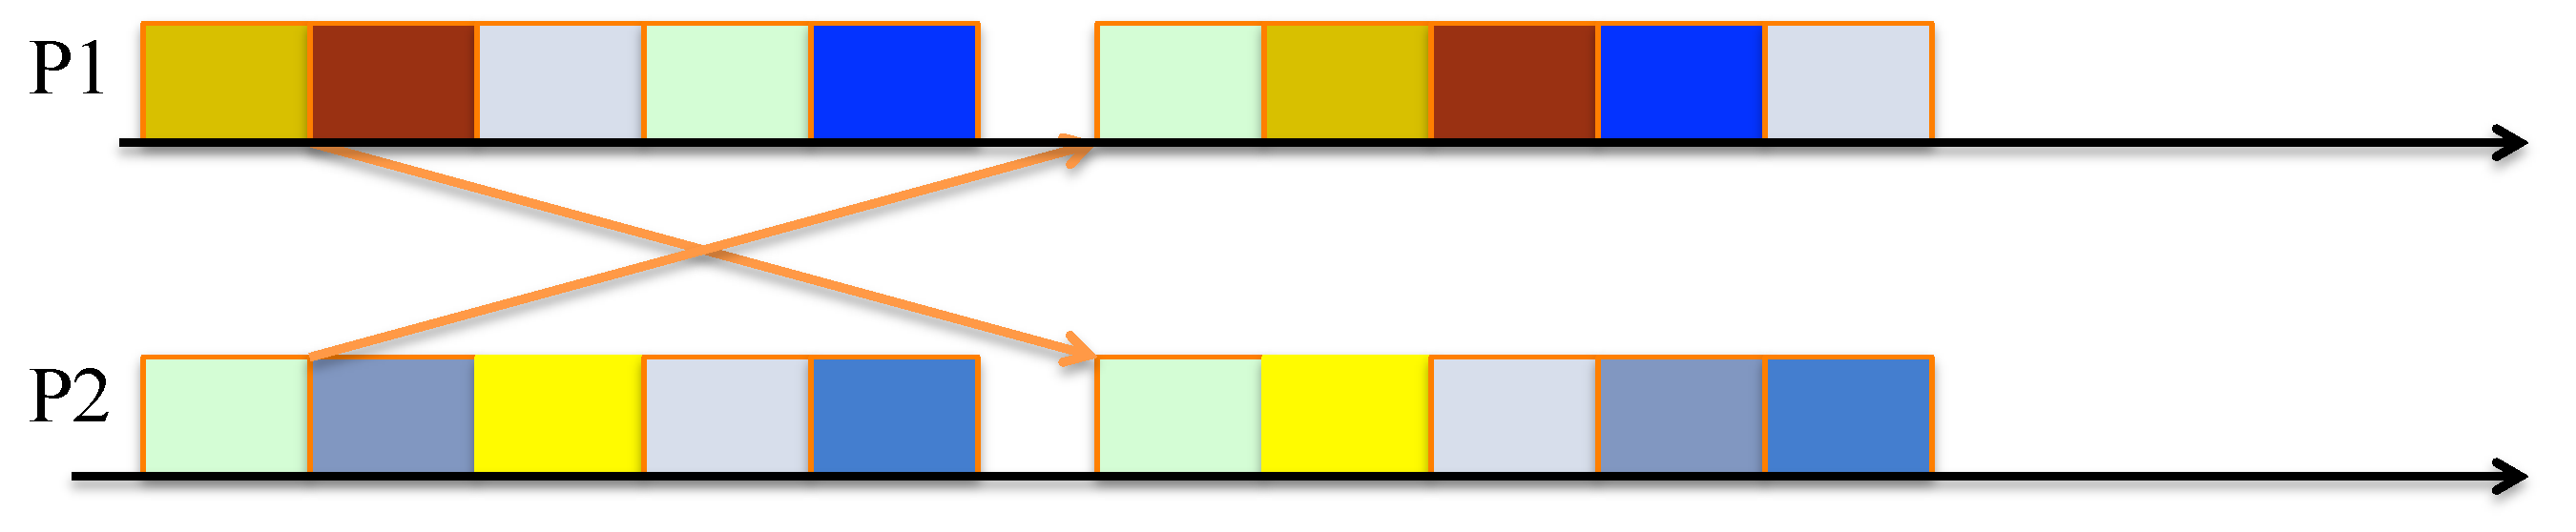
\includegraphics[width=\textwidth]{figures/stencil_timeline2} \end{center}
  \begin{center} Stencil in Charm: Communication of a chare overlaps with
  computation of others \end{center}
\end{frame}

\begin{frame}[t]
\frametitle{Example: Multiple Modules}
Without message-driven execution (and virtualization), you get either: Space-division

  \begin{center} 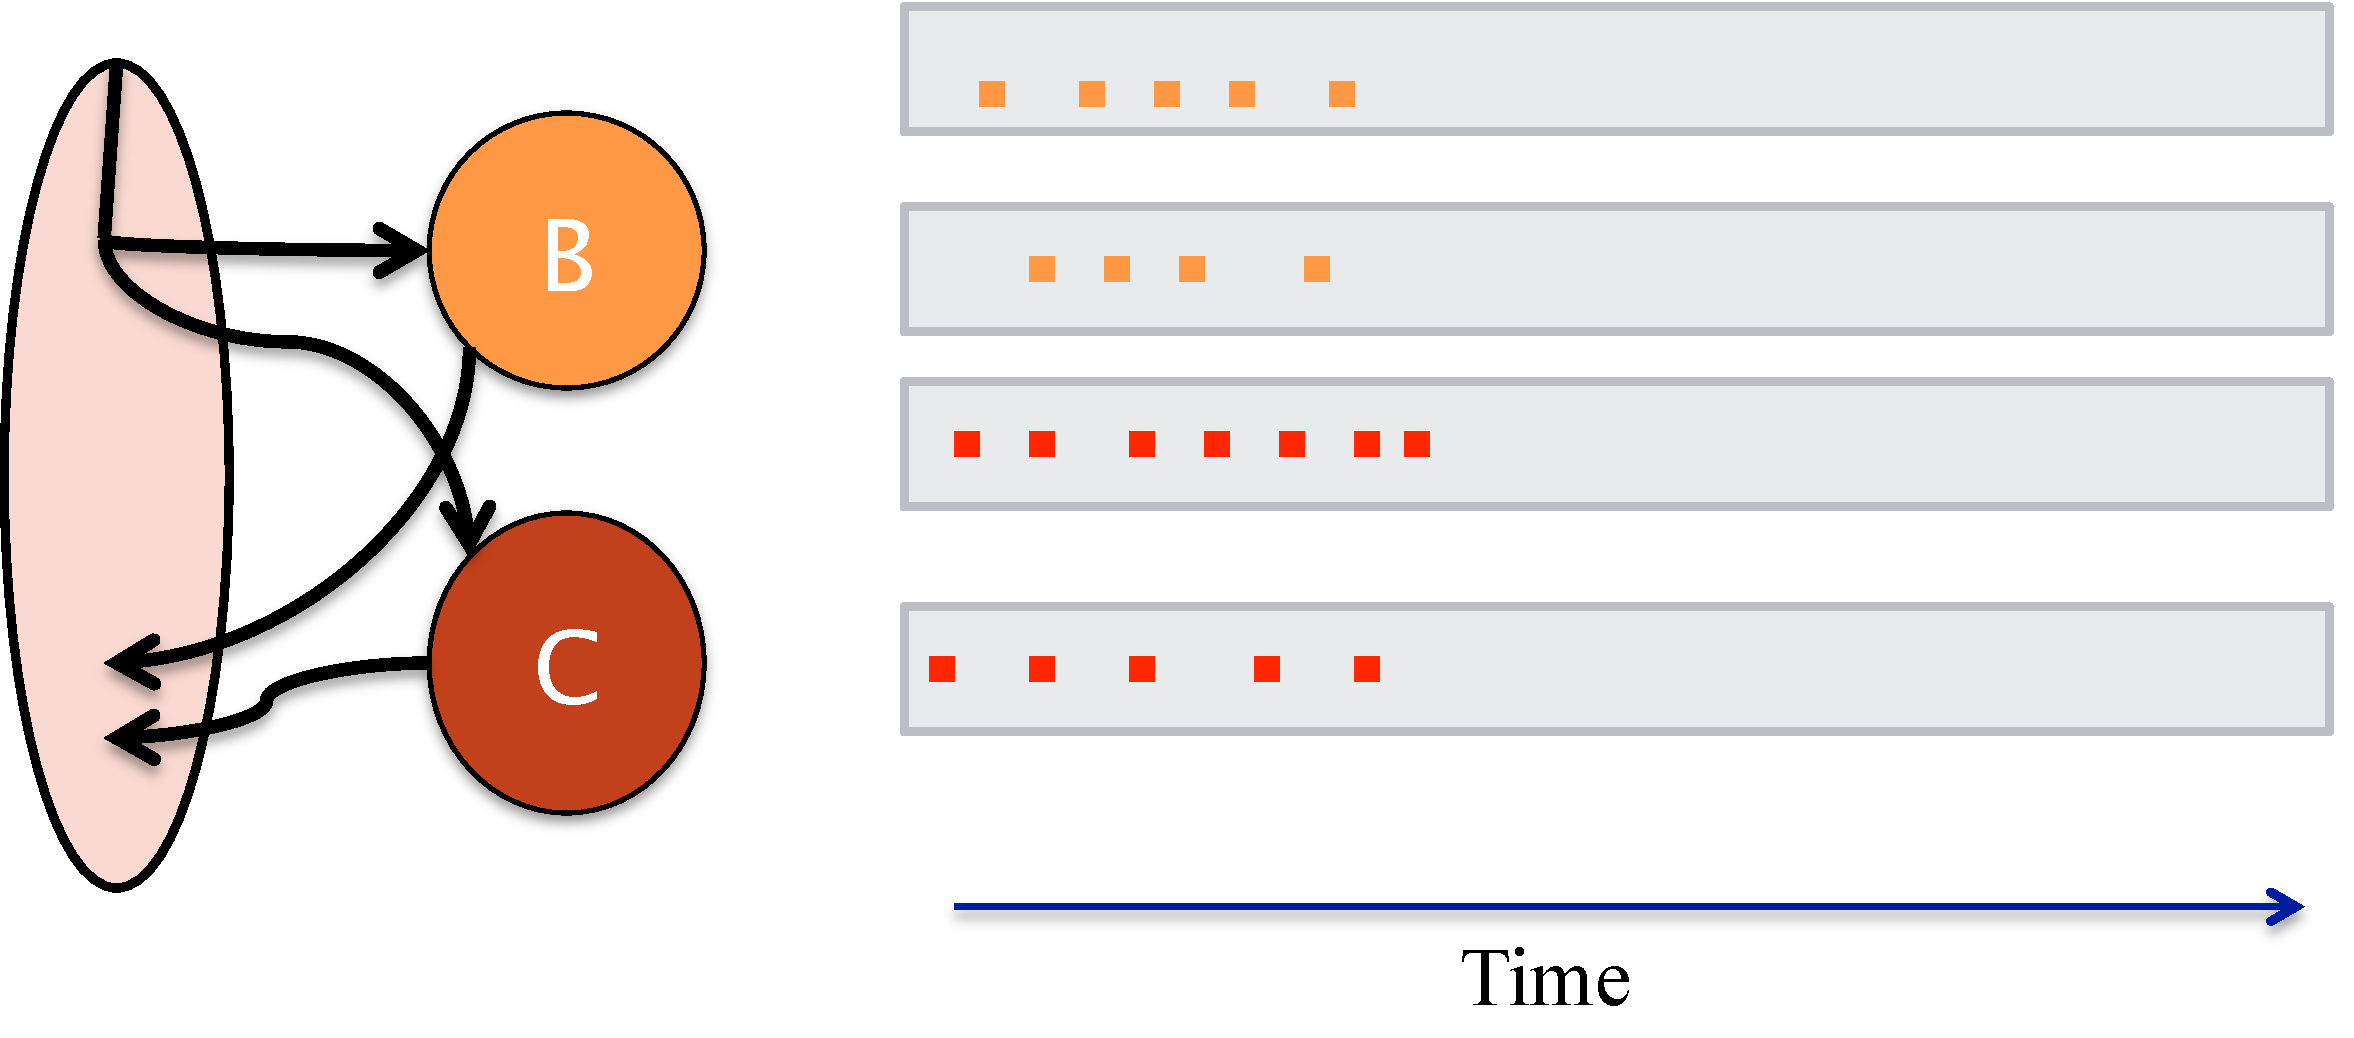
\includegraphics[width=\textwidth]{figures/stencil_space} \end{center}
\end{frame}

\begin{frame}[t]
\frametitle{Example: Multiple Modules}
Sequentialization

  \begin{center} 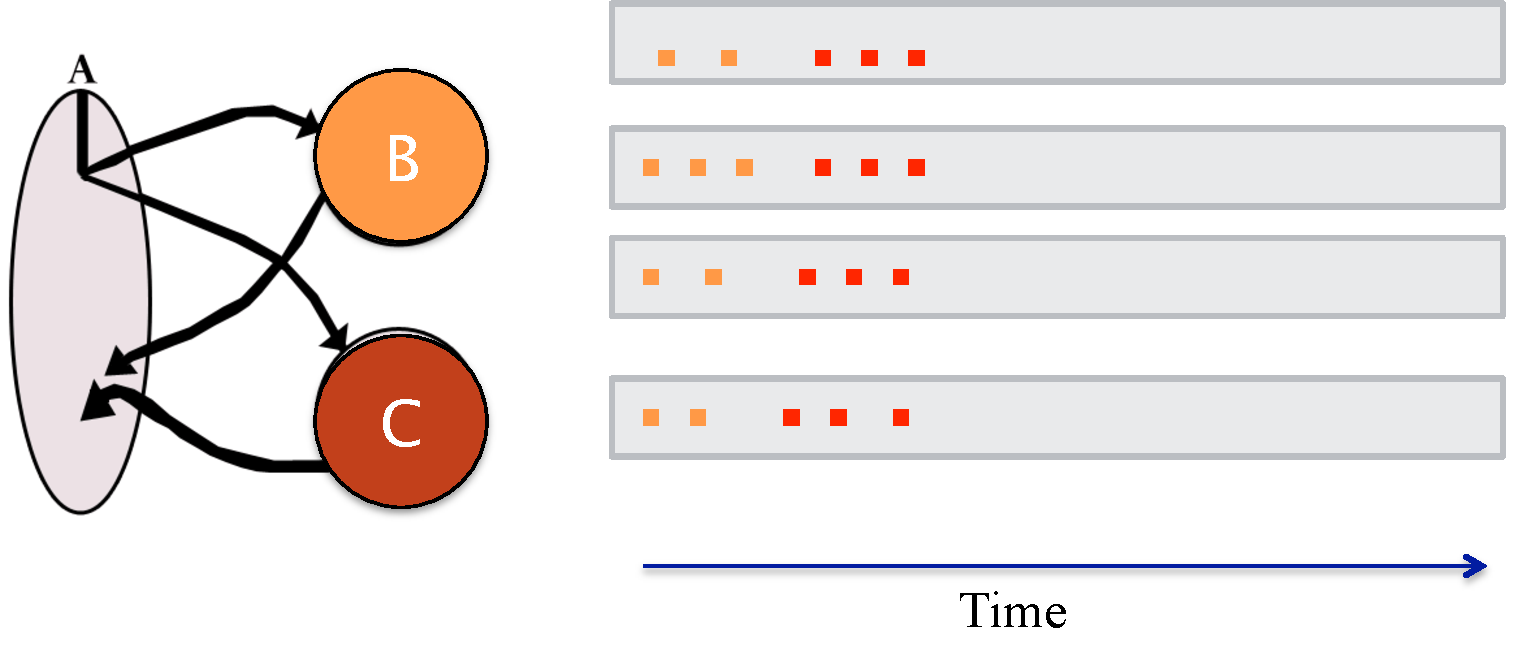
\includegraphics[width=\textwidth]{figures/stencil_seq} \end{center}
\end{frame}

\begin{frame}[t]
\frametitle{Example: Multiple Modules}
Parallel Composition: A1; (B || C ); A2
  \begin{center} 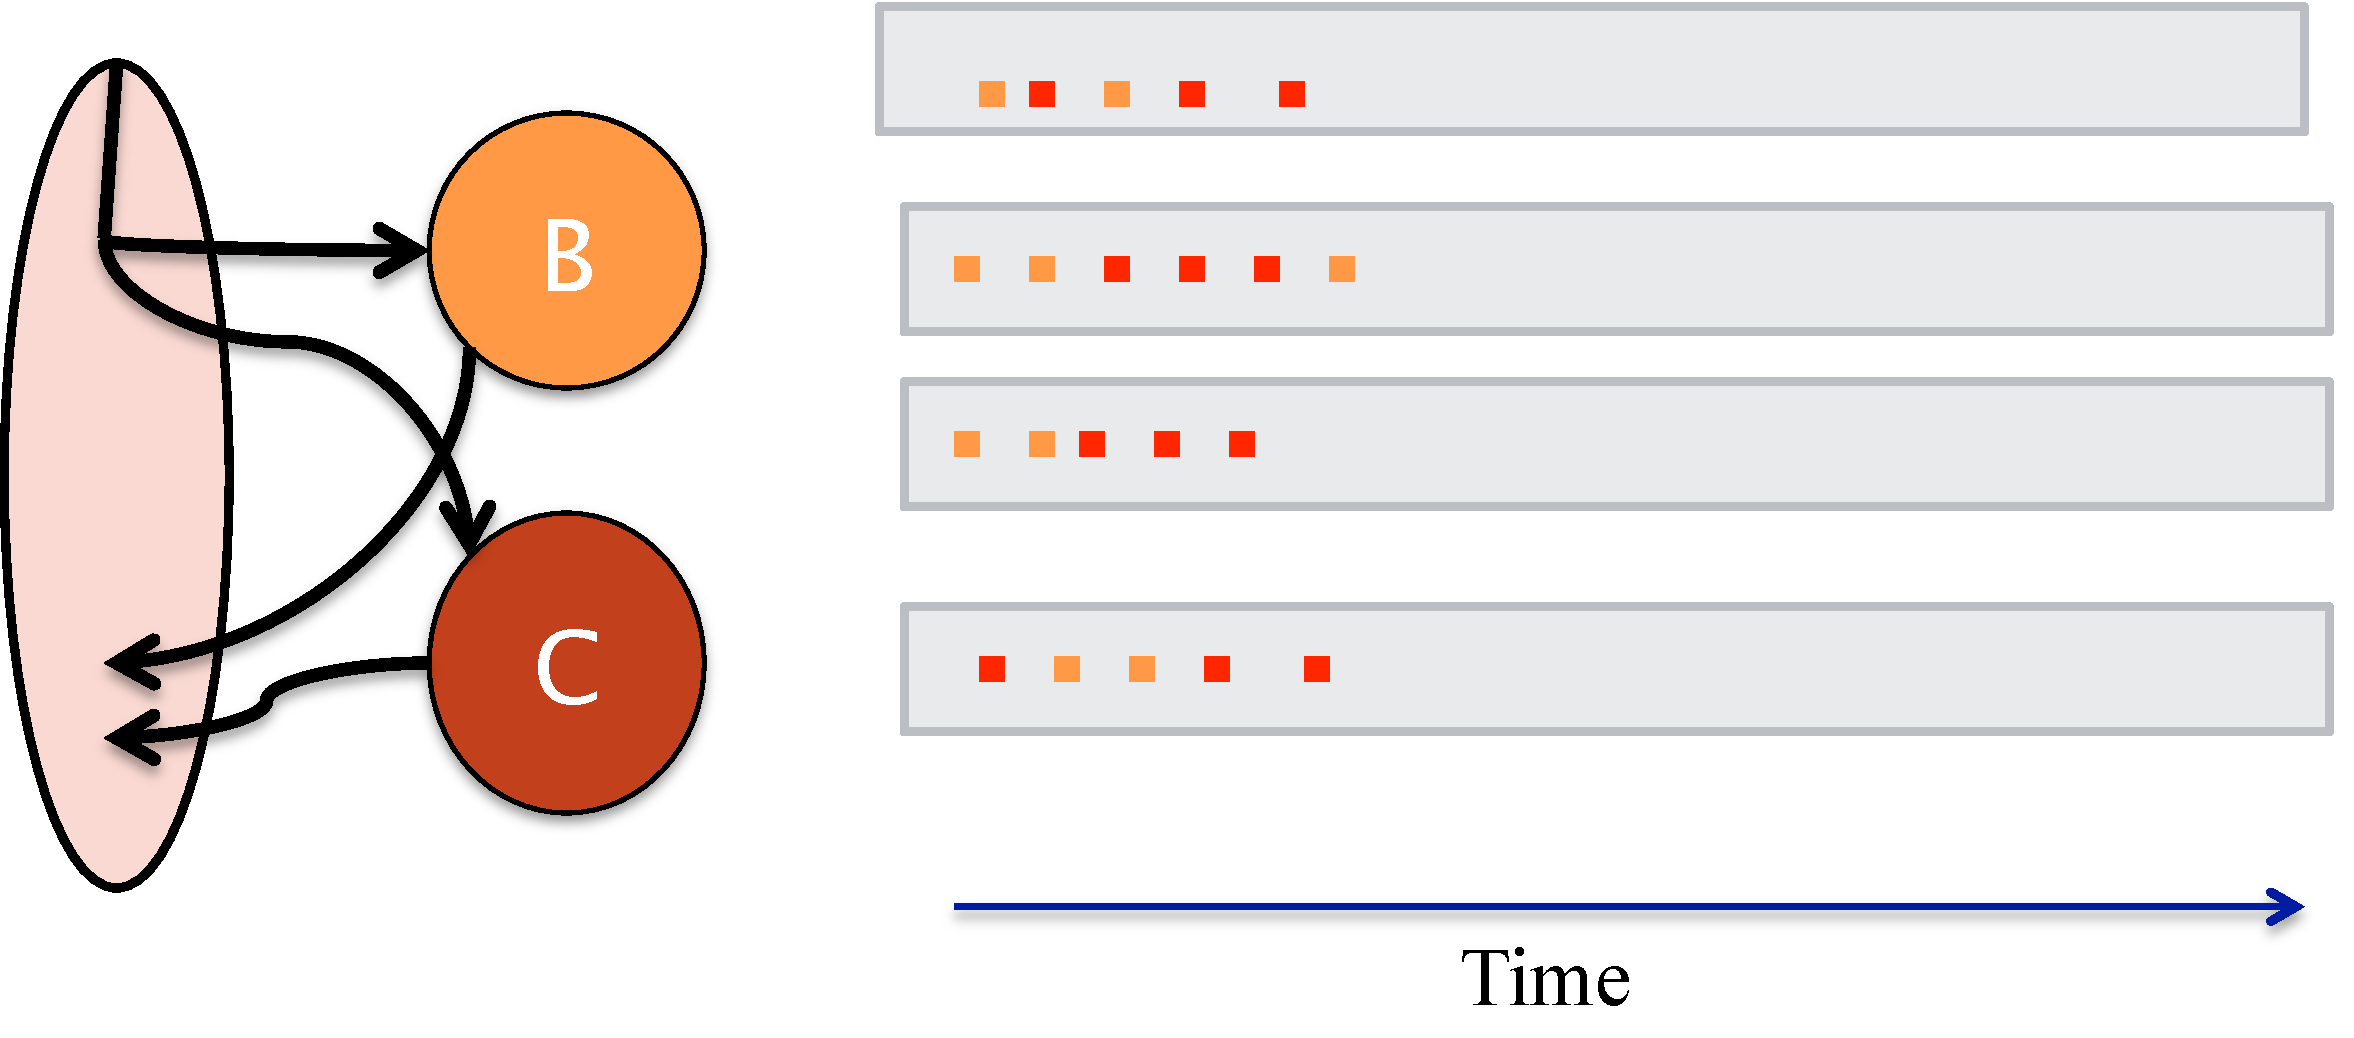
\includegraphics[width=\textwidth]{figures/stencil_charm} \end{center}
Recall: Different modules, written in different languages/paradigms, can overlap
in time and on processors, without programmer having to worry about this
explicitly

\end{frame}

%this is covered in design examples case studies section
%\begin{frame}[t]
%\frametitle{MD Parallelization Using Charm++}
%The computation is decomposed into ``natural'' objects of the application, which
%are assigned to processors by Charm++ RTS
%  \begin{center} 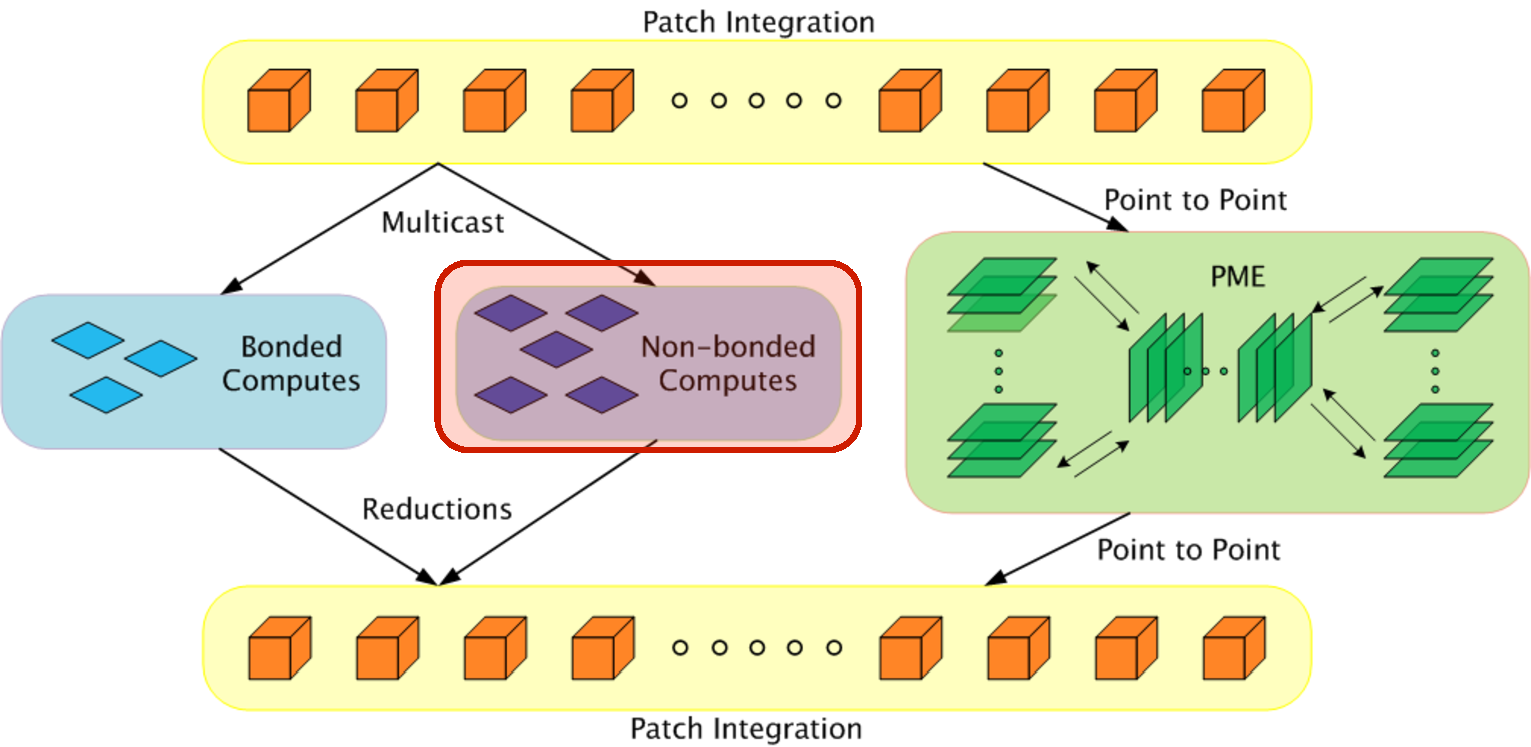
\includegraphics[width=\textwidth]{figures/md_parallelize.pdf}% \end{center}
%\end{frame}

\begin{frame}[t]
\frametitle{Migratability}
  \begin{itemize}
    \item Once the programmer has written the code without reference to
        processors, all of the communication is expressed among objects
    \item The system is free to migrate the objects across processors as and when it pleases
      \begin{itemize}
        \item It must ensure it can deliver method invocations to the objects, whereever they go
        \item This migratability turns out to be a key attribute for empowering an adaptive runtime system
      \end{itemize}
  \end{itemize}
\end{frame}

% TODO: fill in these slides
%\begin{frame}[t]
%  \frametitle{Load Balancing}
%\end{frame}

%\begin{frame}[t]
%  \frametitle{Automatic Overlap of Communication and Computation}
%\end{frame}

%\begin{frame}[t]
%  \frametitle{Fault Tolerance}
%\end{frame}

\begin{frame}[t]
\frametitle{Decomposition Independent of numCores}
  \begin{columns}
    \column{.7\textwidth}
    \begin{itemize}
      \item Rocket simulation under traditional MPI
    \end{itemize}
    \begin{center} 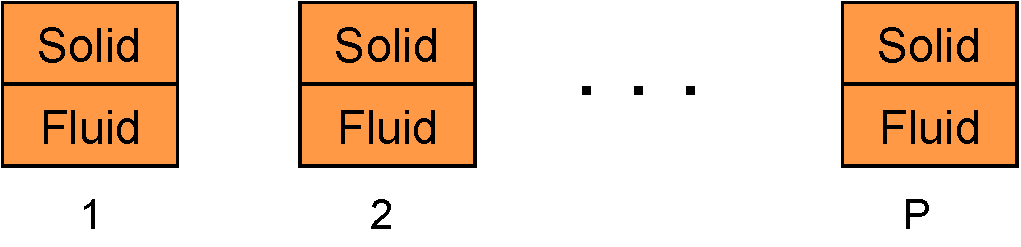
\includegraphics[width=.6\textwidth]{figures/rocket_mpi} \end{center}
    \pause
    \begin{itemize}
      \item Rocket simulation with migratable objects
      \begin{center} 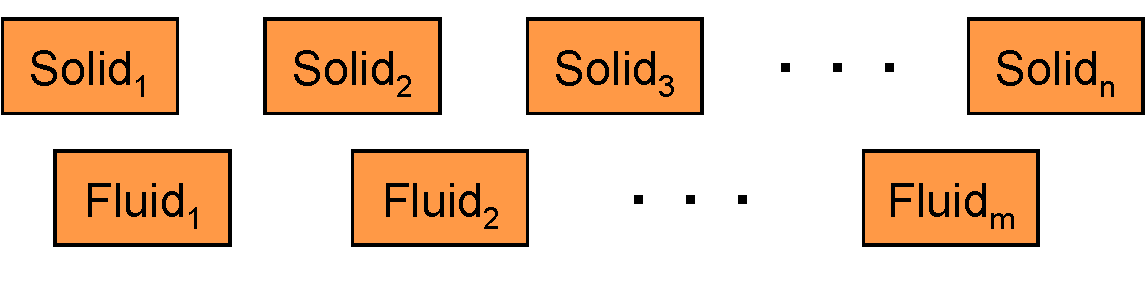
\includegraphics[width=.6\textwidth]{figures/rocket_charm} \end{center}
      \begin{itemize}
        \item Benefits: load balance, communication optimizations, modularity
      \end{itemize}
    \end{itemize}
    \onslide<1-> {
    \column{.3\textwidth}
    \vfill
    \begin{center} \includegraphics<0->[width=\textwidth]{figures/rocket.png} \end{center}
    \vfill
    }
  \end{columns}
\end{frame}
